\documentclass[11pt,a4paper]{article}
\usepackage[margin=24mm,top=24mm,bottom=26mm,headheight=15pt]{geometry}
\usepackage[T1]{fontenc}
\usepackage{newpxtext,newpxmath}
\usepackage{microtype}
\usepackage{amsmath,mathtools}
\usepackage[most]{tcolorbox}
\usepackage{tikz}
\usetikzlibrary{arrows.meta,calc,decorations.pathreplacing,positioning}
\usepackage{xcolor}
\usepackage{fancyhdr}
\usepackage{needspace}
\usepackage{enumitem}
\usepackage{booktabs,array}
\usepackage{caption}
\usepackage{lastpage}
\definecolor{ink}{HTML}{233345}
\definecolor{navy}{HTML}{173A57}
\definecolor{blue}{HTML}{2C6887}
\definecolor{shadeblue}{HTML}{EFF5F8}
\definecolor{sand}{HTML}{F9F4E8}
\definecolor{sandborder}{HTML}{C6B58F}
\definecolor{muted}{HTML}{5D6974}
\definecolor{palegray}{HTML}{E3E8EB}
\definecolor{accent}{HTML}{B76F4F}
\color{ink}
\setlength{\parindent}{0pt}
\setlength{\parskip}{6.2pt plus 1.3pt minus 0.5pt}
\setlength{\abovedisplayskip}{9pt plus 2pt minus 1pt}
\setlength{\belowdisplayskip}{9pt plus 2pt minus 1pt}
\setlength{\abovedisplayshortskip}{7pt}
\setlength{\belowdisplayshortskip}{7pt}
\setlist[itemize]{leftmargin=1.6em,itemsep=2.5pt,topsep=3pt,parsep=0pt}
\setlist[enumerate]{leftmargin=1.8em,itemsep=2.5pt,topsep=3pt,parsep=0pt}
\newcommand{\dd}{\,\mathrm{d}}
\newcommand{\ut}{\frac{\partial u}{\partial t}}
\newcommand{\ux}{\frac{\partial u}{\partial x}}
\newcommand{\highlight}[1]{\textcolor{navy}{#1}}
\newcommand{\secstart}[1]{\Needspace{7\baselineskip}\section{#1}}
\newcommand{\substart}[1]{\Needspace{5\baselineskip}\subsection{#1}}
\newtcolorbox{thinkbox}[1][]{enhanced,breakable,colback=sand,colframe=sandborder,boxrule=.65pt,arc=1.6mm,left=10pt,right=10pt,top=8pt,bottom=8pt,before skip=10pt,after skip=11pt,title={\sffamily\bfseries\small STOP AND THINK},coltitle=navy,fonttitle=\sffamily\bfseries\small,attach boxed title to top left={xshift=9pt,yshift=-2.1mm},boxed title style={colback=sand,colframe=sand,boxrule=0pt},#1}
\newtcolorbox{pointbox}[1][]{enhanced,breakable,colback=shadeblue,colframe=palegray,boxrule=.6pt,arc=1.6mm,left=11pt,right=11pt,top=9pt,bottom=9pt,before skip=12pt,after skip=11pt,#1}
\newcommand{\answer}{\par\smallskip\textbf{Answer.}~}
\newcommand{\captionline}[1]{\begin{center}\small\color{muted}#1\end{center}}
\newcommand{\smalldiv}{\vspace{3pt}\hrule height .45pt\color{palegray}\vspace{6pt}}
\renewcommand{\thesection}{\arabic{section}}
\pagestyle{fancy}
\fancyhf{}
\fancyhead[L]{\scriptsize\sffamily\color{muted} MOVING PATTERN $\longrightarrow$ TRANSPORT EQUATION}
\fancyhead[R]{\scriptsize\sffamily\color{muted} GUIDED DERIVATION}
\fancyfoot[C]{\small\color{muted}\thepage}
\renewcommand{\headrulewidth}{0.3pt}
\renewcommand{\footrulewidth}{0pt}
\setcounter{secnumdepth}{2}
\usepackage{titlesec}
\titleformat{\section}{\Large\bfseries\color{navy}}{\thesection.}{.65em}{}
\titlespacing*{\section}{0pt}{17pt plus 2pt minus 2pt}{7pt}
\titleformat{\subsection}{\normalsize\bfseries\color{navy}}{}{0pt}{}
\titlespacing*{\subsection}{0pt}{12pt}{5pt}
\captionsetup{font=small,labelfont=bf,justification=centering}
\begin{document}
\thispagestyle{fancy}
\vspace*{6mm}
{\centering
{\Huge\bfseries\color{navy} From a Moving Pattern\\[3pt]to the Transport Equation\par}
\vspace{7mm}
{\large\color{muted} A patient derivation, one small step at a time\par}
\vspace{11mm}
{\small\sffamily One moving belt. One rule about where a value came from. One differential equation.\par}
}
\vspace{9mm}
\begin{pointbox}
\textbf{Our destination.} We want to understand why a pattern moving steadily to the right, without stretching or spreading, is described by
\[
\boxed{\displaystyle \ut+c\ux=0,\qquad c>0.}
\]
We will not assume that you know what a partial derivative is, or why there is a minus sign in the argument leading to this equation. We will build the equation from the motion itself.
\end{pointbox}
\vspace{4mm}
\secstart{First picture: a pattern on a moving belt}
Imagine a long conveyor belt painted with a coloured stripe. It moves from \emph{left to right} at a constant speed. The stripe travels with the belt: it does not fade, stretch, or change shape.

A camera above the belt looks at fixed positions along it. At a particular spot, the colour seen by the camera may change as different parts of the painted belt pass underneath. But the stripe itself is unchanged.

\begin{center}
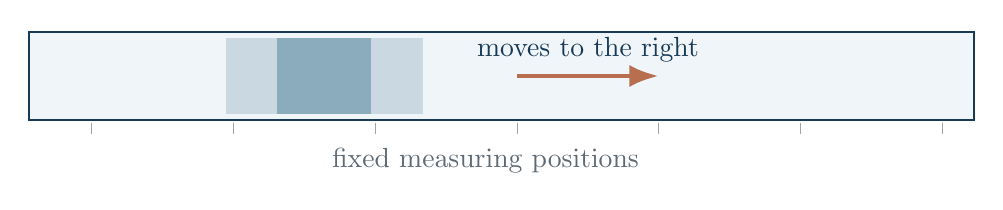
\begin{tikzpicture}[x=1cm,y=1cm,>=Latex]
 \fill[shadeblue] (0,0) rectangle (12,1.12);
 \draw[navy,line width=.9pt] (0,0) rectangle (12,1.12);
 \fill[blue!25] (2.5,.08) rectangle (5.0,1.04);
 \fill[blue!55] (3.15,.08) rectangle (4.35,1.04);
 \draw[->,accent,line width=1.7pt] (6.2,.56)--(8.0,.56);
 \node[above,navy] at (7.1,.62) {moves to the right};
 \foreach \x in {0.8,2.6,4.4,6.2,8,9.8,11.6} {\draw[muted!60] (\x,-.04)--(\x,-.18);}
 \node[below,muted] at (5.8,-.23) {fixed measuring positions};
\end{tikzpicture}
\end{center}
\begin{thinkbox}
If the camera sees the darkest part of the stripe later than before, has the paint become darker?
\answer No. A darker \emph{part of the belt} has arrived at the camera. The pattern is moving; its shape is not changing.
\end{thinkbox}

\clearpage
\secstart{A simple clock-and-grid model}
Before describing every possible position and every instant of time, imagine a deliberately simple version of the belt.

Mark equally spaced measuring sites along the floor, labelled
\[
\ldots,-2,-1,0,1,2,3,\ldots
\]
A clock makes one \emph{tick}. During every tick the belt moves exactly one site to the right. We begin by measuring only at the ticks.

Suppose the painted belt has a dark patch over site $0$ at the start. One tick later that same patch is above site $1$. Another tick later, it is above site $2$.

\begin{center}
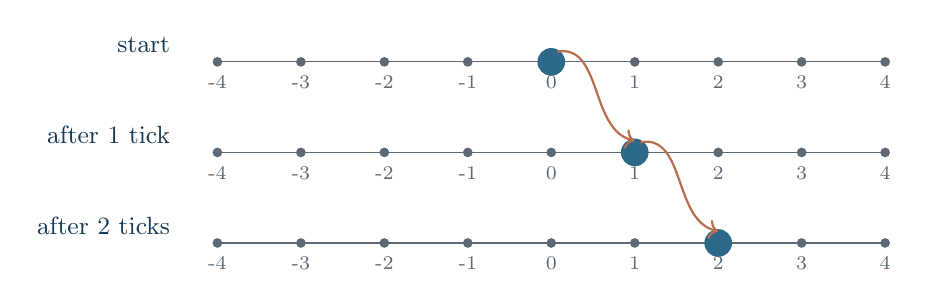
\begin{tikzpicture}[x=1.06cm,y=1cm]
\foreach \yy/\ii/\lab in {2.35/0/{start},1.2/1/{after 1 tick},0.05/2/{after 2 ticks}} {
 \node[anchor=east,navy] at (-.45,\yy+.22) {\small\lab};
 \draw[muted] (0,\yy)--(8,\yy);
 \foreach \j in {0,...,8}{\fill[muted] (\j,\yy) circle (1.75pt); \node[below,muted] at (\j,\yy-.06) {\scriptsize\number\numexpr\j-4\relax};}
 \pgfmathsetmacro{\xx}{4+\ii}
 \fill[blue] (\xx,\yy) circle (5pt);
}
\draw[->,accent,thick] (4.07,2.48) to[out=10,in=168] (5.0,1.35);
\draw[->,accent,thick] (5.07,1.33) to[out=10,in=168] (6.0,.20);
\end{tikzpicture}
\end{center}
The important question is not where a patch \emph{goes}. It is where the patch we see at a chosen site \emph{came from}.

\begin{pointbox}
\textbf{One question to keep asking:} To find what is above site $3$ after the next tick, which site should we inspect \emph{now}?\\
\textbf{Answer:} site $2$, immediately to its left. Everything travels one site to the right.
\end{pointbox}
We shall turn that sentence into a formula. The formula will be exact for our simple moving-belt model.

\begin{thinkbox}
If a marked patch is found at site $-1$ \emph{after} the next tick, where was it \emph{before} the tick?
\answer At site $-2$. Moving right by one carries $-2$ to $-1$.
\end{thinkbox}

\clearpage
\secstart{Name the values, then find the exact rule}
Instead of merely saying ``dark'' or ``light'', give the paint at a site a numerical \emph{intensity}. A value of $0$ means unpainted; larger numbers mean darker paint. These are arbitrary units, not probabilities.

We need a way to say \emph{where} and \emph{when} a particular intensity is measured.
\[
\boxed{U_j^n=\text{paint intensity above site }j\text{ after }n\text{ ticks}.}
\]
The lower label $j$ names the \emph{site}. The upper label $n$ counts the \emph{ticks}. In particular, the small $n$ is \emph{not} an exponent.

Suppose we start with these intensities:
\[
\begin{array}{c|rrrrrrr}
\text{site }j & -2 & -1 & 0 & 1 & 2 & 3 & 4\\\hline
\text{at tick }0:~U_j^0 &0&0&2&5&2&0&0\\
\text{at tick }1:~U_j^1 &0&0&0&2&5&2&0
\end{array}
\]
Look at the $5$: at first it is above site $1$; at the next tick it is above site $2$. The $2$ to its left and the $2$ to its right also move one place. Nothing in the pattern has changed.

\substart{Now choose an arbitrary destination}
We want the intensity at site $j$ \emph{one tick later}. We know only one piece of the belt can arrive there: the piece currently at the site immediately to the left, $j-1$.

So, in words,
\begin{center}\emph{new intensity at $j$ = old intensity at $j-1$.}\end{center}
And in symbols,
\begin{equation}
\boxed{U_j^{n+1}=U_{j-1}^{n}.}\tag{1}
\end{equation}
Read (1) aloud: ``The intensity at site $j$ after $n+1$ ticks equals the intensity at site $j-1$ after $n$ ticks.''

There is \textbf{no approximation} in (1). It follows exactly from the stated rule that the painted belt translates by one site at each tick.

\begin{thinkbox}
Use (1) with $j=2$ and $n=0$. What does it predict about $U_2^1$? Check it against the table.
\answer $U_2^1=U_1^0=5$. This is exactly what the table shows.
\end{thinkbox}

\clearpage
\secstart{Give the sites and ticks physical meaning}
The labels $-2,-1,0,1,2,\ldots$ tell us the order of the sites. They do not yet tell us how far apart the sites are.

Let $h$ be the \emph{distance between two neighbouring sites}, measured, say, in metres. Let $\tau$ (the Greek letter ``tau'') be the \emph{time between two ticks}, measured in seconds.
\[
\boxed{h=\text{distance moved each tick},\qquad
\tau=\text{duration of one tick}.}
\]
These are positive numbers. We write $h>0$ and $\tau>0$.

A site with label $j$ has physical position
\[
\boxed{x=jh.}
\]
A time labelled by tick $n$ has physical time
\[
\boxed{t=n\tau.}
\]
Thus site $j-1$ is not merely ``one index smaller'': it is physically one distance $h$ to the left of $x$, so its coordinate is $x-h$.

\begin{center}
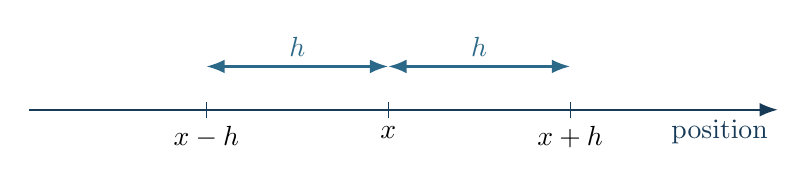
\begin{tikzpicture}[x=1.1cm,y=1cm,>=Latex]
\draw[->,navy,thick] (.25,1.0)--(8.9,1.0) node[below left] {position};
\foreach \x in {2.3,4.4,6.5} {\draw[navy] (\x,.90)--(\x,1.1);}
\node[below] at (2.3,.91) {$x-h$};\node[below] at (4.4,.91) {$x$};\node[below] at (6.5,.91) {$x+h$};
\draw[<->,blue,thick] (2.3,1.55)--(4.4,1.55) node[midway,above] {$h$};
\draw[<->,blue,thick] (4.4,1.55)--(6.5,1.55) node[midway,above] {$h$};
\end{tikzpicture}
\end{center}
\substart{What is the speed of the belt?}
Speed means \emph{distance travelled divided by time taken}. Here the belt goes one distance $h$ in one time interval $\tau$. So its speed, which we name $c$, is
\begin{equation}
\boxed{c=\frac{h}{\tau}.}\tag{2}
\end{equation}
For example, if $h=0.20$ metres and $\tau=0.10$ seconds, the belt covers $0.20$ metres in $0.10$ seconds. Its speed is $2$ metres per second, or $c=2\,\mathrm{m/s}$.

Because the belt moves \emph{right}, we call its signed speed positive: $c>0$. A left-moving belt will be considered in the appendix.

\begin{thinkbox}
Suppose the distance between sites is halved, but we want to describe \emph{exactly the same physical belt speed}. What should happen to the tick duration $\tau$?
\answer It must also be halved. Then $h/\tau$ stays unchanged.
\end{thinkbox}

\clearpage
\secstart{Our most important change: from a grid to a curve}
We have described a sequence of values only at particular sites and particular ticks. A differential equation, however, refers to a value at \emph{every} position and at \emph{every} instant.

We cannot obtain that simply by changing the letters $j$ and $n$ to $x$ and $t$. We have to decide what continuous object the numbers are supposed to approximate.

\substart{A smooth pattern instead of a row of readings}
Imagine that the paint on the belt changes gradually along its length: rather than a sharply edged block of colour, it might become slowly darker and then lighter again. The height of a smooth curve can represent this changing intensity.

We give the curve a name:
\[
\boxed{u(x,t)=\text{intensity at physical position }x\text{ and time }t.}
\]
\begin{center}
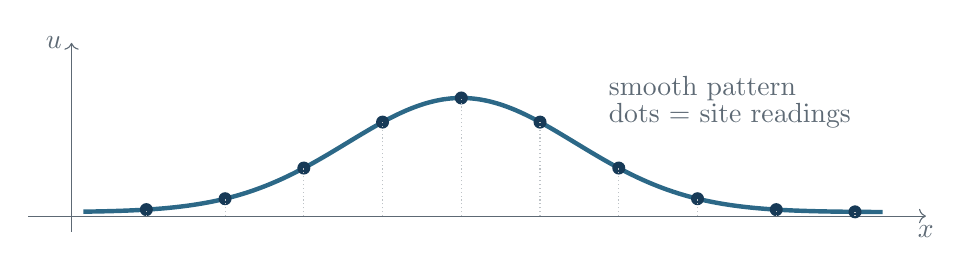
\begin{tikzpicture}[x=1cm,y=1cm]
\draw[->,muted] (0,.2)--(11.4,.2) node[below] {$x$};
\draw[->,muted] (.55,0)--(.55,2.4) node[left] {$u$};
\draw[blue,line width=1.6pt,smooth,samples=90,domain=.7:10.85] plot (\x,{.25+1.45*exp(-0.5*((\x-5.5)/1.45)^2)});
\foreach \x in {1.5,2.5,...,10.5}{
  \pgfmathsetmacro{\val}{.25+1.45*exp(-0.5*((\x-5.5)/1.45)^2)}
  \fill[navy] (\x,\val) circle (2.35pt);
  \draw[muted!40,densely dotted] (\x,.2)--(\x,\val);
}
\node[anchor=west,muted] at (7.25,1.82) {smooth pattern};
\node[anchor=west,muted] at (7.25,1.48) {dots = site readings};
\end{tikzpicture}
\end{center}
\textbf{The crucial assumption.} We assume that at the scale of interest, the moving intensities can be well described by a pattern $u(x,t)$ that changes \emph{smoothly} in space and time. The discrete update rule by itself does not guarantee this. Sharp paint boundaries, for example, are not differentiable everywhere.

In this model the meaning of $U_j^n$ and $u(x,t)$ is the \emph{same kind of physical quantity}: paint intensity. For smooth paint, a grid reading samples the continuous intensity at that location, so we write
\[
U_j^n\;\approx\;u(jh,n\tau).
\]
We use $\approx$ because the continuous profile is our \emph{model} of the recorded values. In an idealisation in which a smooth painted profile exists from the start, the sampling can be exact.

\begin{pointbox}
The job ahead: translate the simple ``comes from one position to the left'' rule into a statement about $u(x,t)$, and \emph{only then} study what happens as $h$ and $\tau$ become small.
\end{pointbox}

\clearpage
\secstart{Translate the rule without losing its meaning}
Recall the exact rule for site values:
\[
U_j^{n+1}=U_{j-1}^{n}.
\]
Take it apart before introducing the smooth pattern.
\begin{itemize}
\item The left side is measured at site $j$ \emph{one tick later}: position $x$, time $t+\tau$.
\item The right side is measured at site $j-1$ \emph{at the current tick}: position $x-h$, time $t$.
\end{itemize}
So the continuous version of the same idea is
\begin{equation}
\boxed{u(x,t+\tau)\;\approx\;u(x-h,t).}\tag{3}
\end{equation}
Say it slowly: ``The intensity I shall see \emph{here} one tick from now is the intensity that is \emph{one step to my left} right now.''

If $u$ represents an ideal smooth pattern being transported rigidly, the shift relation holds with \emph{equality}. If $u$ is only an approximate smooth description of a set of site readings, it is an approximate rule. In the following algebra we use the ideal equality to expose the idea; the continuum interpretation still relies on our smoothness assumption.

\substart{Picture the same shape at two times}
\begin{center}
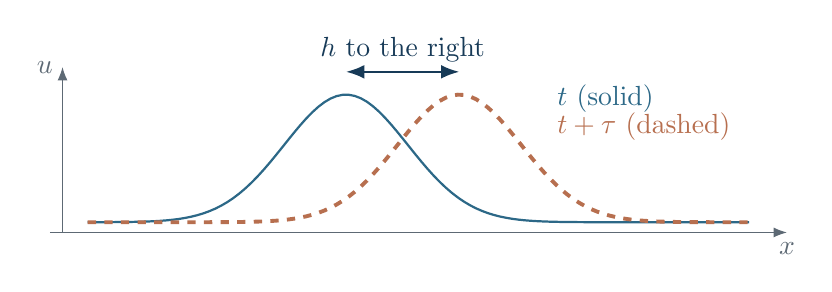
\begin{tikzpicture}[x=.80cm,y=1.0cm,>=Latex]
\def\peakA{5.1}
\draw[->,muted] (.4,.0)--(12.1,.0) node[below] {$x$};
\draw[->,muted] (.6,0)--(.6,2.1) node[left] {$u$};
\draw[blue,thick,samples=110,domain=1.0:11.5] plot (\x,{.13+1.62*exp(-.52*(\x-5.1)^2)});
\draw[accent,dashed,line width=1.4pt,samples=110,domain=1.0:11.5] plot (\x,{.13+1.62*exp(-.52*(\x-6.9)^2)});
\draw[<->,navy,thick] (5.1,2.04)--(6.9,2.04) node[midway,above] {$h$ to the right};
\node[blue,anchor=west] at (8.3,1.7) {$t$ (solid)};
\node[accent,anchor=west] at (8.3,1.35) {$t+\tau$ (dashed)};
\end{tikzpicture}
\end{center}
\captionline{Same height, same width: the whole profile shifts one distance $h$ to the right.}

The peak has moved, but its height has not. The same is true of every part of the curve. \emph{Translation} is not the same as \emph{spreading}. We shall check the precise meaning of the minus sign in the next picture.

\begin{thinkbox}
Why is the earlier location $x-h$ rather than $x+h$?
\answer Because the belt moves to the right. The piece that reaches $x$ must have started to its \emph{left}.
\end{thinkbox}

\clearpage
\secstart{Focus on one fixed position}
The previous picture shows a whole curve moving. Now keep your eye on \emph{one fixed physical position} $x$.

\begin{center}
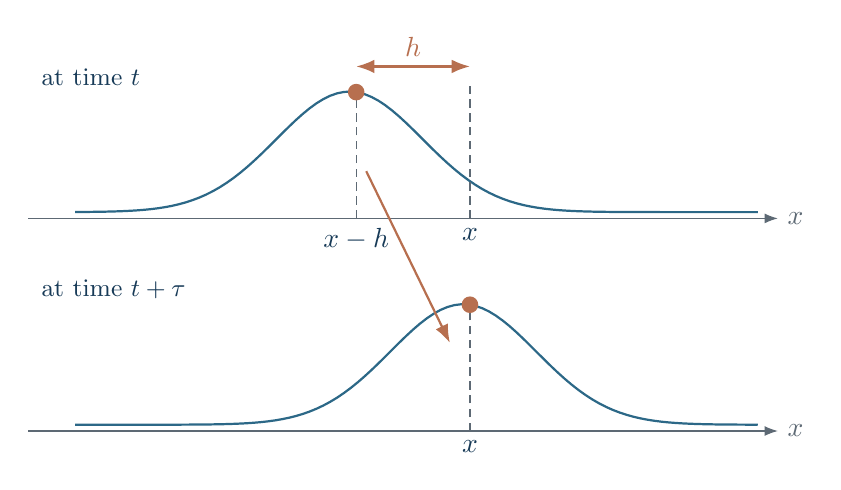
\begin{tikzpicture}[x=.85cm,y=1.0cm,>=Latex]
\def\xx{7.0}
\foreach \yy/\shift/\titletext in {2.8/0/{at time $t$},.1/1.7/{at time $t+\tau$}} {
 \draw[->,muted] (.4,\yy)--(11.6,\yy) node[right] {$x$};
 \draw[blue,thick,samples=100,domain=1.1:11.3] plot (\x,{\yy+.08+1.53*exp(-.42*(\x-5.2-\shift)^2)});
 \node[anchor=west,navy] at (0.45,\yy+1.8) {\small\titletext};
 \draw[muted,densely dashed] (7,\yy)--(7,\yy+1.75);
}
\draw[muted,densely dashed] (5.3,2.8)--(5.3,4.45);
\draw[<->,accent,thick] (5.3,4.73)--(7.0,4.73) node[midway,above] {$h$};
\node[below,navy] at (5.3,2.8) {$x-h$};
\node[below,navy] at (7,2.8) {$x$};
\node[below,navy] at (7,.1) {$x$};
\fill[accent] (5.3,{2.8+.08+1.53*exp(-.42*(5.3-5.2)^2)}) circle (3pt);
\fill[accent] (7,{.1+.08+1.53*exp(-.42*(7-6.9)^2)}) circle (3pt);
\draw[->,accent,thick] (5.45,3.4)--(6.7,1.22);
\end{tikzpicture}
\end{center}
The orange dot at $x-h$ on the earlier curve becomes the orange dot at $x$ on the later curve. Those dots have the \emph{same height} because they represent the same painted part of the belt.

This is precisely what
\[
u(x,t+\tau)=u(x-h,t)
\]
says. The two arguments of $u$ have different meanings: the \emph{first} specifies where we look, and the \emph{second} specifies when we look.

\begin{thinkbox}
If a transition from darker paint on the left to lighter paint on the right approaches a stationary camera, can the intensity seen by the camera increase even though the paint never changes?
\answer Yes. More strongly painted parts are arriving at the camera. The change is caused by motion past a fixed point, not by paint changing on the belt.
\end{thinkbox}

\clearpage
\secstart{First algebraic step: isolate what changes}
We are now ready for the main calculation. Start with the ideal shift rule:
\begin{equation*}
u(x,t+\tau)=u(x-h,t).
\end{equation*}
This compares values at \emph{different} places and times. We want to reveal two simpler comparisons: the change in time at one fixed place, and the change in space at one fixed time.

\substart{Subtract the old value at $x$}
Subtract $u(x,t)$ from \emph{both} sides. We are allowed to do this because subtracting the same number from each side preserves equality.
\begin{equation}
\boxed{u(x,t+\tau)-u(x,t)=u(x-h,t)-u(x,t).}\tag{4}
\end{equation}
Look at the \emph{left}: the location $x$ is identical in both terms. Only the time has changed. So the left side is ``new intensity minus old intensity at the \emph{same} camera.''

Look at the \emph{right}: the time $t$ is identical in both terms. Only the position has changed. So the right side compares two neighbouring places along the belt.

\begin{pointbox}
\textbf{Why subtract?} A differential equation tells us about \emph{changes}. Equation (4) has made the time change visible on the left and the spatial change visible on the right.
\end{pointbox}
\substart{Divide by the duration of one tick}
To turn the left-hand change into a \emph{rate of change}, divide by the time interval $\tau$. Again, we must divide \emph{both} sides:
\begin{equation}
\boxed{\frac{u(x,t+\tau)-u(x,t)}{\tau}
=\frac{u(x-h,t)-u(x,t)}{\tau}.}\tag{5}
\end{equation}
The left side is the \emph{average change in intensity per second} over the next tick, at position $x$.

The right side still has time in the denominator, although its numerator compares \emph{positions}. We shall separate the speed of the belt from the slope of the paint pattern.

\begin{thinkbox}
If the left side of (5) is positive, what happened to the intensity seen at the fixed camera during that tick?
\answer It increased: the later value was larger than the earlier value.
\end{thinkbox}

\clearpage
\secstart{Second algebraic step: expose the spatial slope}
We want the right side of (5) to contain a familiar distance-based calculation: change in intensity divided by change in position.

Recall that the distance between the two neighbouring points is $h$. Multiply and divide the right side by $h$. We have changed nothing, since $h/h=1$:
\[
\frac{u(x-h,t)-u(x,t)}{\tau}
=\frac{h}{\tau}\cdot\frac{u(x-h,t)-u(x,t)}{h}.
\]
There is just one awkward feature. For the usual left-to-right slope, we prefer \emph{right height minus left height}. That means reversing the order of the two terms.

Reversing a subtraction changes its sign. For ordinary numbers,
\[
2-5=-(5-2).
\]
The same is true of these two intensities:
\[
u(x-h,t)-u(x,t)=-\bigl[u(x,t)-u(x-h,t)\bigr].
\]
Put both steps into (5). Our equation becomes
\begin{equation}
\boxed{\frac{u(x,t+\tau)-u(x,t)}{\tau}
=-\frac{h}{\tau}\,\frac{u(x,t)-u(x-h,t)}{h}.}\tag{6}
\end{equation}
\textbf{Read each part.} The first fraction measures a \emph{time change per second}. The last fraction measures a \emph{spatial change per metre}. The factor $h/\tau$ is the speed $c$ from (2).

So we can also write
\begin{equation}
\frac{u(x,t+\tau)-u(x,t)}{\tau}
=-c\,\frac{u(x,t)-u(x-h,t)}{h}.
\tag{7}
\end{equation}
No derivatives have been used so far: this is just subtraction, division, and the motion rule.

\begin{thinkbox}
If the intensity increases as we walk from left to right, is $u(x,t)-u(x-h,t)$ positive or negative? Then what does (7) predict for the time change at a fixed camera?
\answer The spatial difference is positive. Since $c>0$, the right side of (7) is negative: the camera sees a decreasing intensity as the rising part of the pattern passes to its right.
\end{thinkbox}

\clearpage
\secstart{What happens when the steps become tiny?}
We have a correct equation for finite steps and a smooth ideal belt. But our destination is an equation involving values at a single instant and a single position. We approach that by making the site spacing and tick duration smaller.

\substart{First: the time change}
Hold the position $x$ fixed. Focus on the left side of (7):
\[
\frac{u(x,t+\tau)-u(x,t)}{\tau}.
\]
This is ``change in intensity divided by the elapsed time''. If the change is smooth, making $\tau$ smaller brings the average rate closer and closer to the \emph{instantaneous} rate of change at time $t$.

That limiting rate is written
\begin{equation*}
\lim_{\tau\to0}\frac{u(x,t+\tau)-u(x,t)}{\tau}
=\frac{\partial u}{\partial t}(x,t).
\end{equation*}
The symbol $\partial u/\partial t$ means: \emph{change time while holding the position fixed}. It is the time derivative of a function that depends on both position and time.

\substart{Second: the change across space}
Now hold the time $t$ fixed. Look at the last fraction in (7):
\[
\frac{u(x,t)-u(x-h,t)}{h}.
\]
The numerator is the height at the \emph{right} position minus the height at the \emph{left} position. The denominator is the distance between them. So this is the slope of a small section of the profile.

If the profile is smooth, letting $h$ shrink makes that secant slope approach the slope of the curve at $x$:
\begin{equation*}
\lim_{h\to0}\frac{u(x,t)-u(x-h,t)}{h}
=\frac{\partial u}{\partial x}(x,t).
\end{equation*}
The symbol $\partial u/\partial x$ means: \emph{change position while holding the time fixed}. It is the spatial derivative.

\begin{pointbox}
\textbf{Two different comparisons.} The left quotient follows one camera through a short \emph{time}. The right quotient surveys two cameras separated by a short \emph{distance}. The transport equation tells us how those two measurements are related.
\end{pointbox}

\clearpage
\secstart{One more condition: keep the speed the same}
There is a final, essential detail. We want to study the \emph{same physical motion} as our measuring grid becomes finer. If $h$ shrinks but $\tau$ does not, we have made the belt slower. If $\tau$ shrinks much faster than $h$, we have made it faster.

So we make $h$ and $\tau$ smaller \emph{together}, keeping their ratio equal to (or approaching) a fixed positive speed $c$:
\begin{equation}
\boxed{h\longrightarrow0,\qquad \tau\longrightarrow0,
\qquad\frac{h}{\tau}\longrightarrow c>0.}\tag{8}
\end{equation}
For example, all three of the following descriptions represent speed $c=2$ metres per second:
\[
\begin{array}{c|c|c}
\text{distance per tick }h & \text{seconds per tick }\tau & h/\tau\\\hline
0.20 & 0.10 & 2\\
0.10 & 0.05 & 2\\
0.02 & 0.01 & 2
\end{array}
\]
Each row describes a finer way of tracking motion at the \emph{same speed}.

\substart{Now, and only now, combine the limits}
Return to the equation that we derived by ordinary algebra:
\[
\frac{u(x,t+\tau)-u(x,t)}{\tau}
=-\frac{h}{\tau}\,\frac{u(x,t)-u(x-h,t)}{h}.
\]
We have examined all three pieces separately:
\begin{itemize}
\item the left fraction tends to $\partial u/\partial t$;
\item the middle factor $h/\tau$ tends to the fixed speed $c$;
\item the final fraction tends to $\partial u/\partial x$.
\end{itemize}
Under our smoothness and scaling assumptions, their limiting relationship is therefore
\begin{equation*}
\frac{\partial u}{\partial t}=-c\frac{\partial u}{\partial x}.
\end{equation*}
Add $c\,\partial u/\partial x$ to both sides:
\begin{equation}
\boxed{\displaystyle\frac{\partial u}{\partial t}
+c\frac{\partial u}{\partial x}=0,\qquad c>0.}\tag{9}
\end{equation}
This is the \textbf{one-dimensional transport equation}, also called the \emph{advection equation}.

\clearpage
\secstart{Does the equation say the right thing?}
Before trusting any mathematical model, check whether its predictions match our original physical picture.

The equation can be read as
\[
\underbrace{\frac{\partial u}{\partial t}}_{\substack{\text{change at one}\\\text{fixed camera}}}
=-c\,\underbrace{\frac{\partial u}{\partial x}}_{\substack{\text{slope of the pattern}\\\text{at one instant}}}.
\]
\textbf{A downward slope.} Imagine that, from left to right, the paint becomes \emph{lighter}. Then $u_x<0$. Because $c>0$, the equation gives $u_t=-cu_x>0$. The fixed camera sees intensity \emph{increase}: darker paint from the left is arriving. That is what a right-moving belt should do.

\textbf{An upward slope.} If the pattern becomes darker from left to right, then $u_x>0$, so $u_t<0$. The camera sees intensity \emph{decrease}: lighter paint arrives from the left.

\textbf{A flat portion.} If $u_x=0$ at a smooth point, then $u_t=0$ there at that instant. The camera sees no instantaneous change in intensity.

\begin{center}
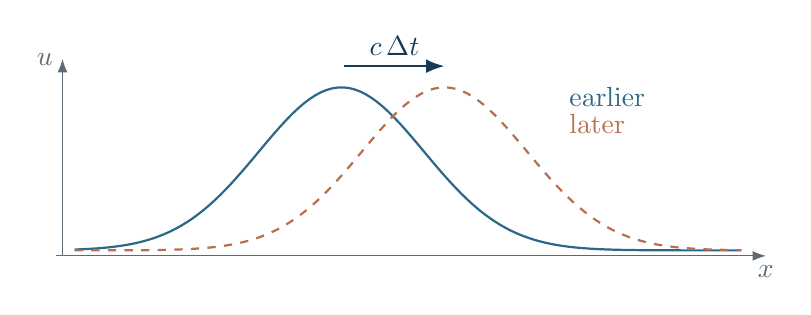
\begin{tikzpicture}[x=.77cm,y=1cm,>=Latex]
\draw[->,muted] (.6,.2)--(12.3,.2) node[below] {$x$};
\draw[->,muted] (.7,.2)--(.7,2.7) node[left] {$u$};
\draw[blue,thick,samples=120,domain=.9:11.9] plot (\x,{.27+2.07*exp(-.27*(\x-5.3)^2)});
\draw[accent,dashed,thick,samples=120,domain=.9:11.9] plot (\x,{.27+2.07*exp(-.27*(\x-7.0)^2)});
\node[blue,anchor=west] at (8.9,2.22) {earlier};
\node[accent,anchor=west] at (8.9,1.88) {later};
\draw[->,navy,thick] (5.35,2.61)--(7.0,2.61) node[midway,above] {$c\,\Delta t$};
\end{tikzpicture}
\end{center}
\captionline{A pulse travels right. Unlike the heat equation, it does not flatten or widen.}

\begin{thinkbox}
At the top of the smooth pulse, $u_x=0$. Does that mean the whole pulse has stopped moving?
\answer No. Only the \emph{instantaneous height at that fixed position} is not changing as the peak passes. The complete profile continues to translate.
\end{thinkbox}

\clearpage
\secstart{A check using a travelling shape}
We have already derived the transport equation. We can now verify the result in a second way. This is a \emph{check}, not a substitute for the discrete-to-continuous argument.

Let $f$ name the painted pattern at the starting time. Thus $f(z)$ means the intensity at position $z$ \emph{on the belt's initial pattern}. After time $t$, a belt moving at speed $c$ has shifted by distance $ct$.

To find the intensity now at $x$, look back to the place $x-ct$ where that piece of belt began. So the moving pattern has the form
\begin{equation}
\boxed{u(x,t)=f(x-ct).}\tag{10}
\end{equation}
At $t=0$, this reads $u(x,0)=f(x)$, the initial paint pattern. At a later time the \emph{same function} is evaluated at a shifted location: this is why its shape does not change.

\substart{Check the time derivative}
Write $z=x-ct$ to shorten the argument. Suppose $f$ is differentiable; its derivative is written $f'(z)$.

The chain rule says: if $u=f(z)$ and $z$ changes, the rate of change of $u$ is the slope $f'(z)$ times the rate of change of $z$.

When $x$ is fixed and $t$ varies, $z=x-ct$ changes at rate $-c$. So
\[
\frac{\partial u}{\partial t}=-c\,f'(x-ct).
\]
\substart{Check the spatial derivative}
When $t$ is fixed and $x$ varies, $z=x-ct$ changes at rate $1$. The same chain rule therefore gives
\[
\frac{\partial u}{\partial x}=f'(x-ct).
\]
Substitute those two expressions into the left side of (9):
\[
\frac{\partial u}{\partial t}+c\frac{\partial u}{\partial x}
= -c f'(x-ct)+c f'(x-ct)=0.
\]
\textbf{It works.} Any differentiable pattern $f$ translated at constant speed $c$ satisfies the transport equation.

\begin{thinkbox}
If the initial pattern has its highest point at $x=4$ and the speed is $c=3$ metres per second, where is the highest point after $2$ seconds?
\answer At $x=4+3\times2=10$ metres. Every feature moves the same distance $ct=6$ metres.
\end{thinkbox}

\clearpage
\secstart{What was exact, and what was assumed?}
Keeping these distinctions clear is more important than memorising the final formula.

\begin{enumerate}
\item \textbf{Exact within the clock-and-grid model.} If each labelled piece of belt moves exactly one site to the right at each tick without changing its painted intensity, then $U_j^{n+1}=U_{j-1}^n$ is exact.
\item \textbf{An additional modelling choice.} We assume the painted intensity can be represented by a smooth function $u(x,t)$ on the length and time scales of interest. A series of arbitrary site readings does not automatically give a differentiable curve.
\item \textbf{A relation inherited from motion.} A smooth profile undergoing rigid translation obeys $u(x,t+\tau)=u(x-h,t)$ whenever the displacement during $\tau$ is $h$. For smooth approximations to cell readings the corresponding relation is approximate.
\item \textbf{A limiting step.} We let $h$ and $\tau$ become small, and assume the relevant difference quotients approach derivatives.
\item \textbf{A fixed physical speed.} The ratio $h/\tau$ must approach a finite positive constant $c$. That is what keeps the physical motion unchanged as our measurements become finer.
\end{enumerate}
\begin{pointbox}
\textbf{The whole argument in four lines}\par\smallskip
\begin{align*}
\text{move right one site:}\quad &U_j^{n+1}=U_{j-1}^n,\\[2pt]
\text{smooth moving pattern:}\quad &u(x,t+\tau)\approx u(x-h,t),\\[2pt]
\text{compare the changes:}\quad &\frac{u(x,t+\tau)-u(x,t)}{\tau}
\approx-\frac{h}{\tau}\frac{u(x,t)-u(x-h,t)}{h},\\[2pt]
\text{tiny steps, fixed speed:}\quad &\boxed{u_t+c\,u_x=0.}
\end{align*}
\end{pointbox}
\substart{Transport versus heat}
In your earlier random-walk derivation, the particle could jump both left and right. That rule involves \emph{two neighbours} and, in the appropriate small-step limit, produces a \emph{second spatial derivative}. It describes spreading.

Here we have only one incoming neighbour: the one on the left. Our rule produces a \emph{first spatial derivative}. It describes translation without spreading. The difference begins in the discrete physical rules, \emph{before} any calculus.

\clearpage
\section*{Appendix A. What if we start from a particle?}
\addcontentsline{toc}{section}{Appendix A. What if we start from a particle?}
A one-particle story can reach the same equation, but it requires a little extra care because a particle at a known starting location does not make a smooth probability profile.

\substart{The deterministic motion is simple}
Suppose a particle jumps one site to the right at each tick. A particle starting at site $0$ visits sites $1,2,3,\ldots$. If its starting site is known, there is no randomness in its later position.

But suppose we \emph{do not know} its starting site. Perhaps the particle starts at $-1$ with probability $1/4$, at $0$ with probability $1/2$, or at $1$ with probability $1/4$. These three possibilities all move one place right on the next tick:
\[
\begin{array}{c|rrrrr}
\text{site }j&-1&0&1&2&3\\\hline
\text{initial probability}&1/4&1/2&1/4&0&0\\
\text{after one tick}&0&1/4&1/2&1/4&0
\end{array}
\]
Let $p_j^n$ denote the probability of finding the particle at site $j$ after $n$ ticks. To be at site $j$ next tick, it must have been at $j-1$ this tick. The particle definitely moves right, so
\[
\boxed{p_j^{n+1}=p_{j-1}^{n}.}
\]
This is the same one-neighbour rule as for the painted belt. It is exact.

\substart{A probability at one site is not a continuous density}
There is one important difference from paint intensity. If we make grid sites closer together, the probability assigned to a \emph{single} site generally becomes smaller. A smooth probability \emph{density} $u$ is scaled so that, roughly speaking, the probability attached to one narrow site of width $h$ is
\[
p_j^n\approx h\,u(jh,n\tau).
\]
We do not need integrals to understand the factor: a cell half as wide carries roughly half as much probability when the underlying density is smooth.

Both sides of the exact update have the \emph{same factor} $h$. When we substitute the smooth approximation, it cancels, leaving the same approximate shift rule for $u$.

\textbf{Important limit of this argument.} A particle starting at one exactly known point remains concentrated at a single position. It does not turn into a differentiable density merely because the steps are small. A smooth initial probability profile is an additional assumption. This is why the painted-belt example is the cleaner main derivation.

\clearpage
\section*{Appendix B. Left-moving patterns and the sign}
Suppose instead that the belt moves one site \emph{left} at each tick. To find what arrives at site $j$ after the next tick, we must look to its \emph{right}, at site $j+1$.

The exact discrete rule becomes
\[
U_j^{n+1}=U_{j+1}^{n}.
\]
In physical coordinates the shift relation is
\[
u(x,t+\tau)=u(x+h,t).
\]
Subtract $u(x,t)$ from both sides, then divide by $\tau$:
\[
\frac{u(x,t+\tau)-u(x,t)}{\tau}
=\frac{h}{\tau}\frac{u(x+h,t)-u(x,t)}{h}.
\]
Now the right spatial quotient already points from left to right; no minus sign is needed. With $h/\tau\to c>0$ and differentiability, this gives
\[
\boxed{\ut-c\ux=0\qquad\text{(leftward speed }c\text{).}}
\]
Alternatively, use a \emph{signed velocity} $v$. Then the single formula $u_t+v u_x=0$ covers both directions: $v>0$ means right; $v<0$ means left.

\section*{Appendix C. What if each jump is random?}
Suppose a particle jumps one site right with probability $r$ and one site left with probability $1-r$. Each new jump is independent of the past. Its starting position may also be uncertain.

To arrive at $j$ on the next jump, there are now \emph{two} possible routes. It can arrive from $j-1$ by jumping right, or from $j+1$ by jumping left. The probabilities of these mutually exclusive routes add:
\[
\boxed{p_j^{n+1}=r\,p_{j-1}^{n}+(1-r)\,p_{j+1}^{n}.}
\]
If $r=1$, every jump goes right and the second term disappears: we recover our pure transport rule. If $r=1/2$, there is no preferred direction, and the usual heat-equation scaling gives spreading instead.

If $r$ is fixed as $h$ and $\tau$ shrink with $h/\tau\to v>0$, the average displacement in one tick is $rh-(1-r)h=(2r-1)h$. Dividing by the tick duration gives the average velocity
\[
\boxed{c=(2r-1)v.}
\]
Under suitable smoothness assumptions, the spreading effect is of smaller order with this \emph{fixed-speed} scaling, so the leading limiting law is $u_t+c u_x=0$. The heat equation uses a different balance, with $h^2/\tau$ remaining finite; do not mix the two scalings.

\clearpage
\section*{Appendix D. Questions worth returning to}
\substart{1. What if $h\to0$ but $\tau$ stays fixed?}
Then $h/\tau\to0$. The belt covers less and less distance per tick, while ticks are still the same duration. The physical motion slows towards zero. It is \emph{not} the same moving belt described with better precision.

\substart{2. Could a pattern translate but also become taller?}
Yes, but it would no longer obey our model. The exact belt rule assumes every marked piece retains its intensity. Growth or fading would require another term in the equation. Pure transport describes an unchanged profile in motion.

\substart{3. Why is the spatial derivative first order?}
The discrete rule compares the value at $x$ with the value at \emph{one neighbouring position}, $x-h$. Subtracting and dividing by $h$ yields one slope. The symmetric random walk instead combines \emph{both} $x-h$ and $x+h$; the relevant difference is a change \emph{between slopes}, which leads to a second derivative.

\substart{4. Must the profile be smooth everywhere?}
Not for transport to be meaningful. A sharp-edged paint stripe can move unchanged. But the classical derivative manipulations in the main text require differentiability at the point under discussion. More advanced courses explain how to treat sharp edges using weaker notions of solution.

\substart{5. What information specifies a particular moving pattern?}
The equation states the \emph{rule of motion}. We must also be given the initial shape $u(x,0)=f(x)$. Then, for a constant speed $c$, the translated pattern is $u(x,t)=f(x-ct)$, at points where the classical derivatives exist.

\begin{pointbox}
\textbf{The essential message.} A value seen at a fixed location next moment came from an earlier location one step to the left. When that one-step translation is examined over tiny distances and times at a fixed speed, the simple rule becomes
\[
\boxed{u_t+c\,u_x=0.}
\]
\end{pointbox}
\vfill
\begin{center}\small\color{muted} End of guided derivation\end{center}
\end{document}
